\documentclass[11pt]{article}

\usepackage{graphicx}
\usepackage{amssymb}
\usepackage{amsfonts}
\usepackage{amsmath}

\setlength{\parindent}{0pt}

\begin{document}

\section*{Aerodynamic simulation in SolidWorks Flow dink}

Solidworks flow simulation for a simplified version of the tandem trike (simple wheels, no chairs).
Increased ``global initial mesh refinement'' until results converge.

It is clear that predicted force $F$, and power $P$ calculated by $P = F v$ is low by a factor $\approx 3$. 

\begin{table}[h!]
\centering
\begin{tabular}{ | l | r | }
\hline
  & Drag (N) \\ \hline
 no roof & 15.9   \\
 flat roof & 17.0 \\
 curved roof & 19.1 \\
 curved roof and sidefenders & 18.5 \\
 covered front & 34.3 \\
 covered front and sidefenders & 30.6 \\ \hline
\end{tabular}
\caption{Drag force for wind speed of 10m/s, for different roof shapes}
\end{table}

\begin{figure}[h!]
\centering
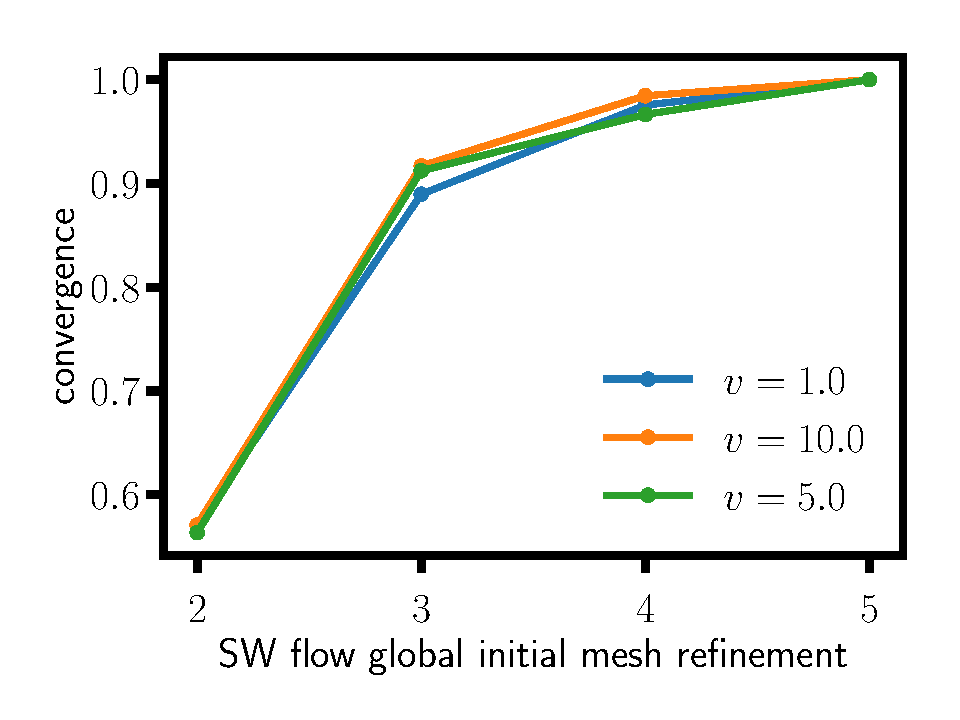
\includegraphics[width=0.55\textwidth]{convergence.pdf}
\end{figure}

\begin{figure}[h!]
\centering
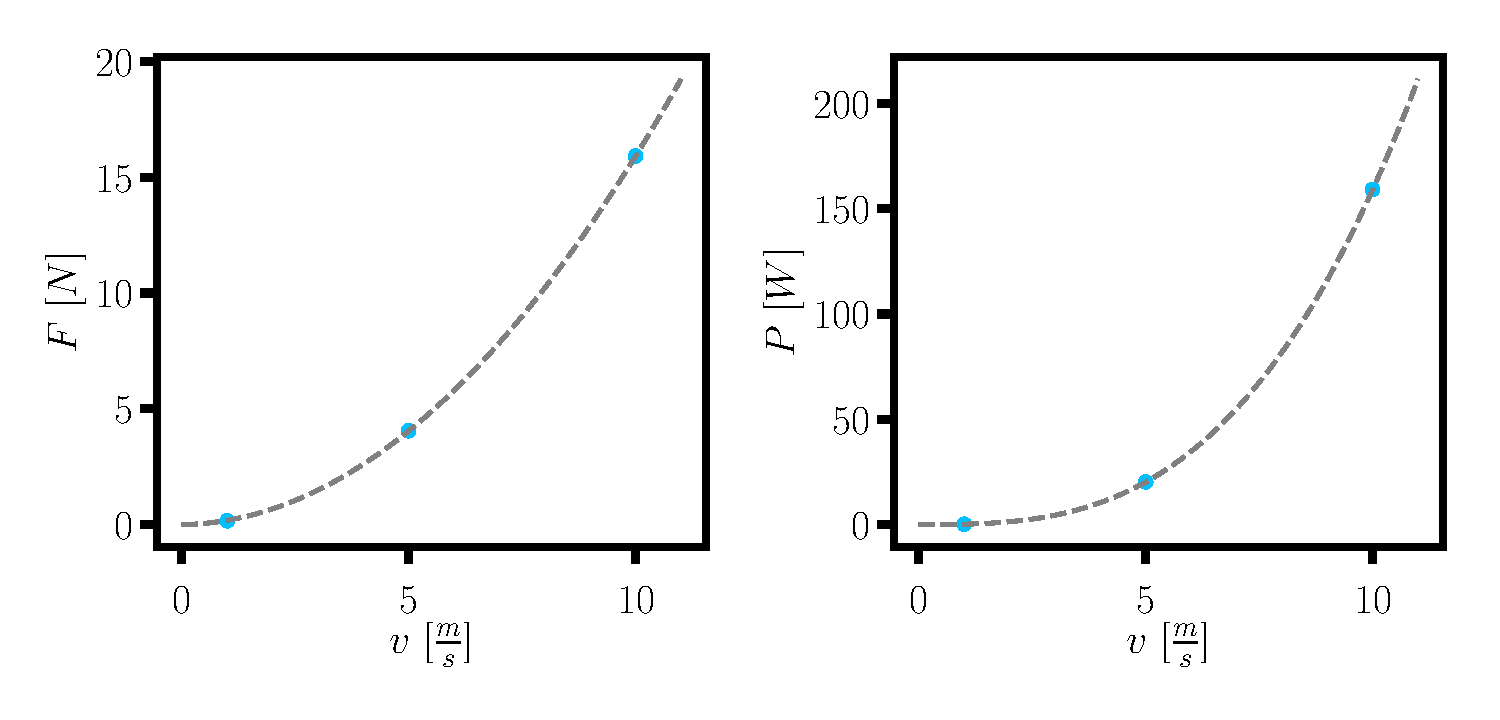
\includegraphics[width=\textwidth]{ForcePower.pdf}
\end{figure}

\section*{Sideview velocity contour plots}

\begin{figure}
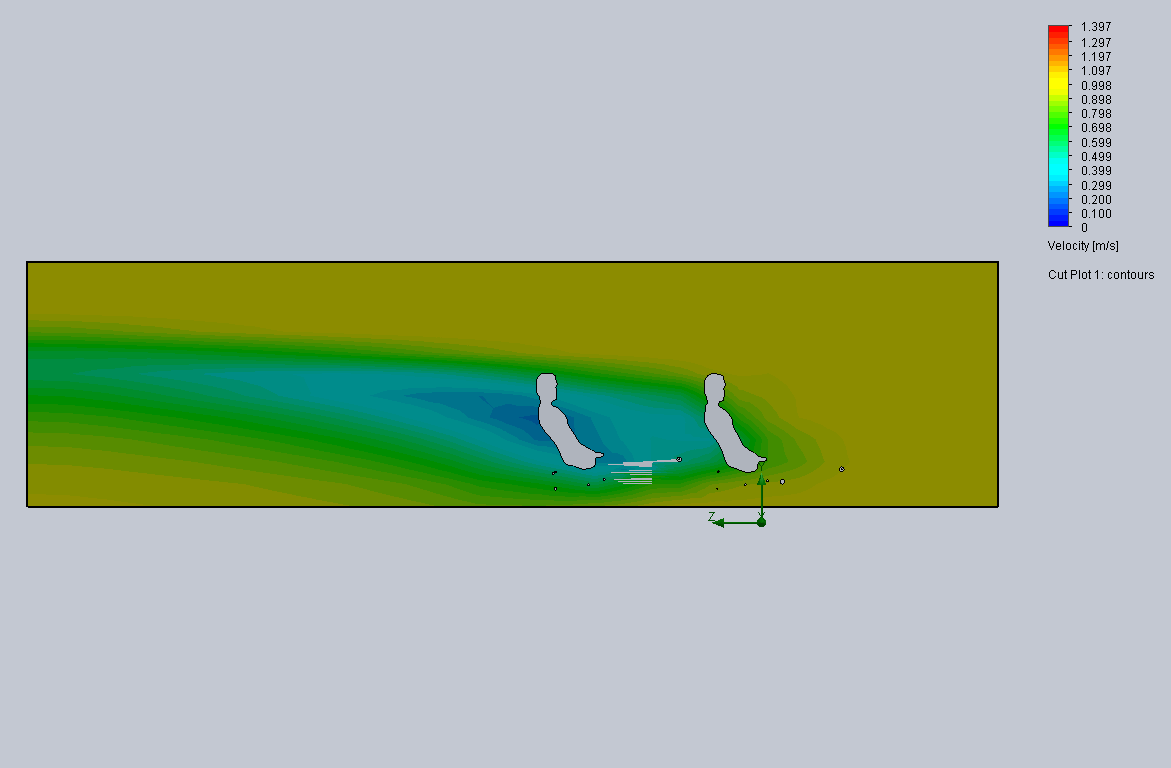
\includegraphics[width=\textwidth]{gm_2_rf_7_v01.png}
\caption{$v = 1 m/s$, global initial mesh = 2}
\end{figure}

\begin{figure}
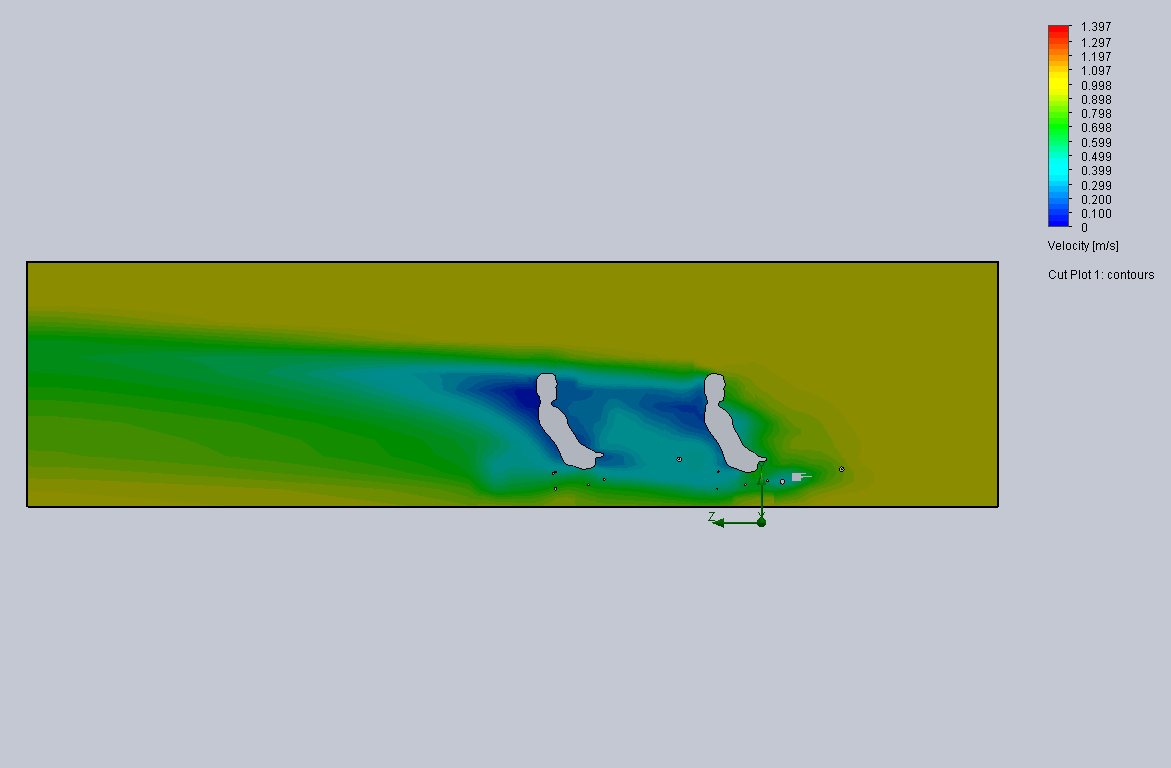
\includegraphics[width=\textwidth]{gm_3_rf_7_v01.png}
\caption{$v = 1 m/s$, global initial mesh = 3}
\end{figure}

\begin{figure}
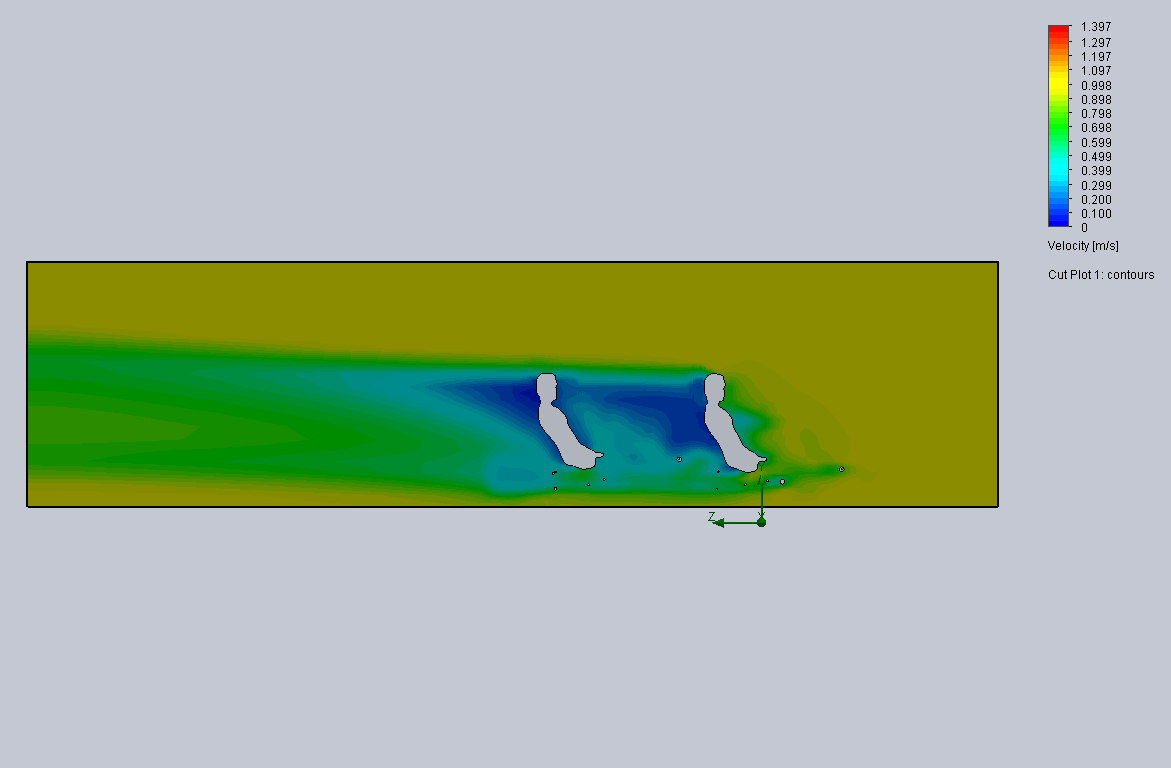
\includegraphics[width=\textwidth]{gm_4_rf_7_v01.png}
\caption{$v = 1 m/s$, global initial mesh = 4}
\end{figure}

\begin{figure}
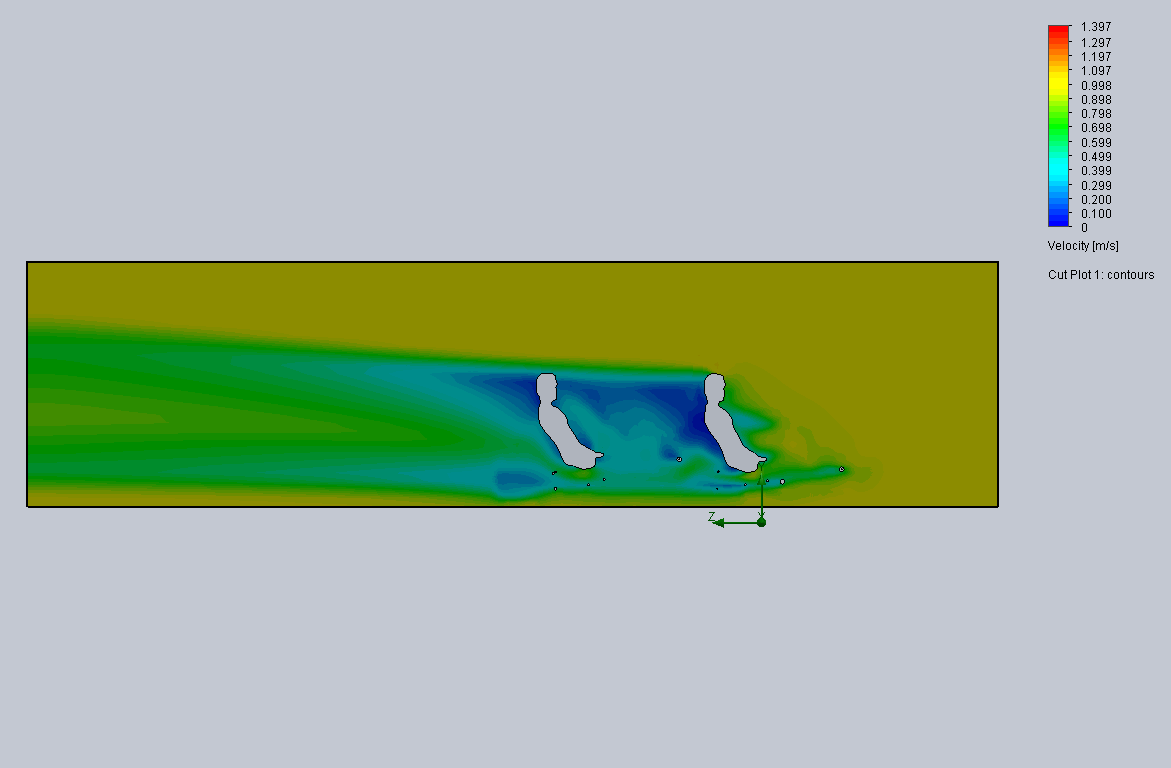
\includegraphics[width=\textwidth]{gm_5_rf_7_v01.png}
\caption{$v = 1 m/s$, global initial mesh = 5}
\end{figure}


\begin{figure}
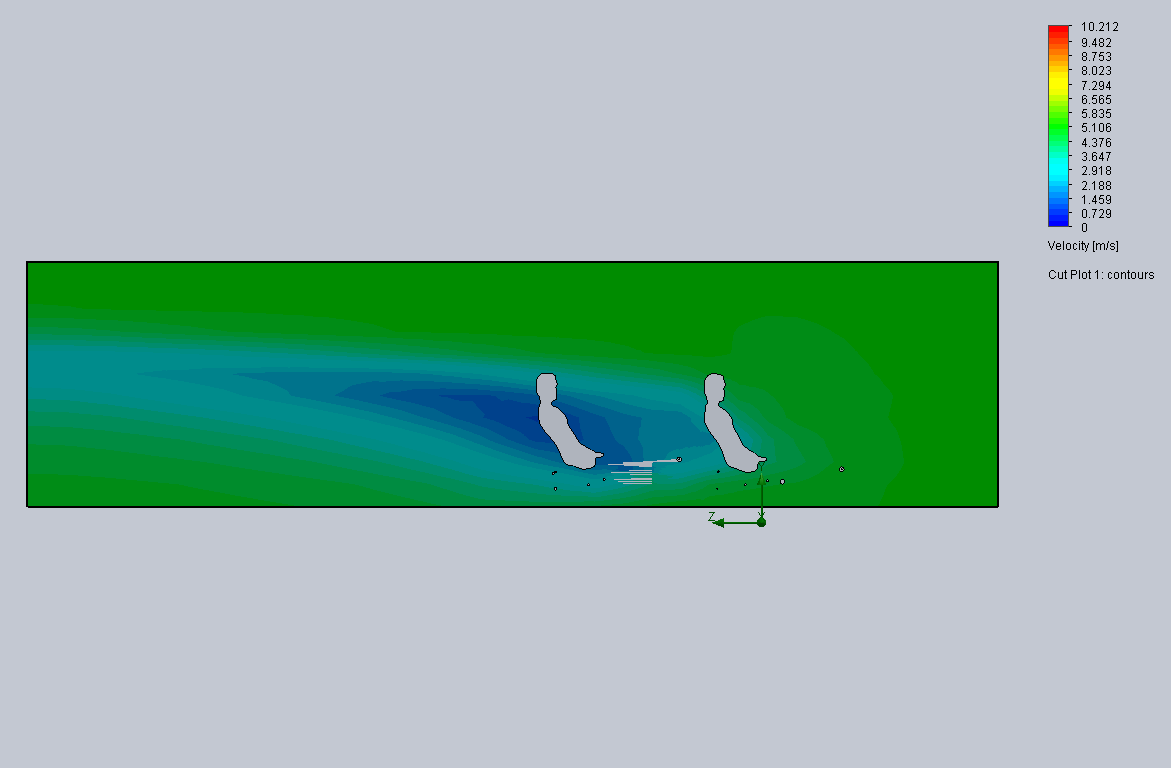
\includegraphics[width=\textwidth]{gm_2_rf_7_v05.png}
\caption{$v = 5 m/s$, global initial mesh = 2}
\end{figure}

\begin{figure}
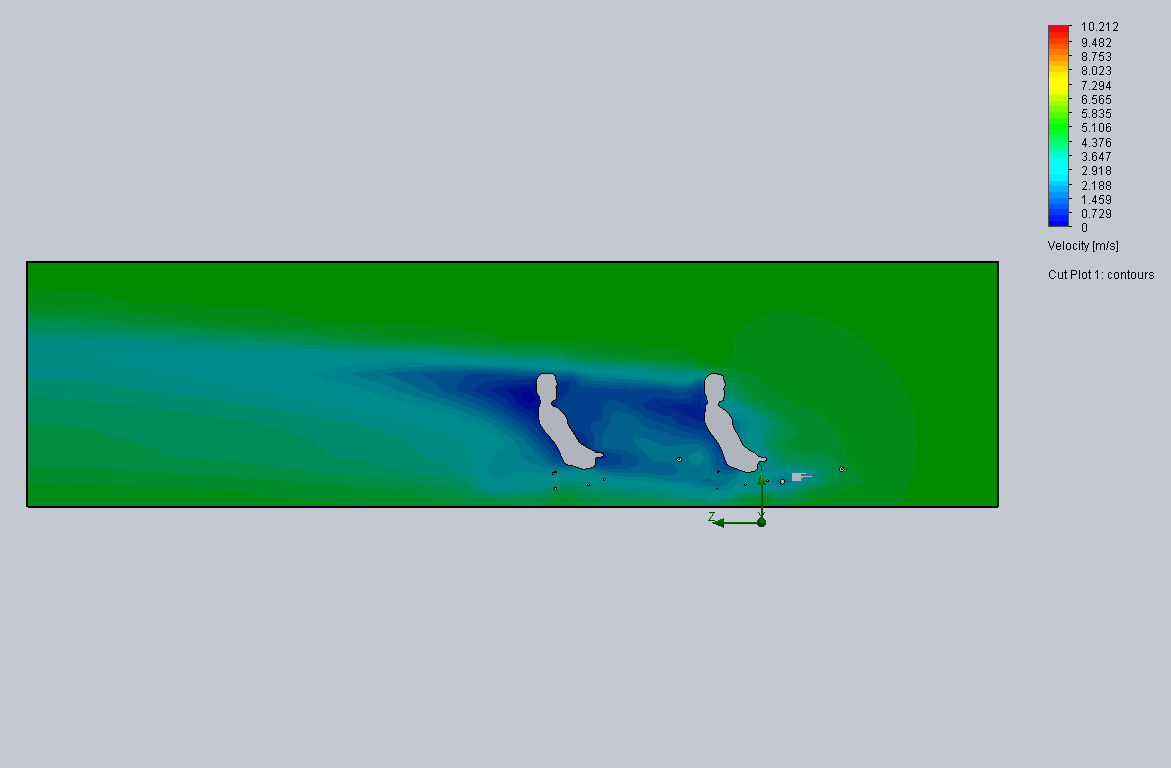
\includegraphics[width=\textwidth]{gm_3_rf_7_v05.png}
\caption{$v = 5 m/s$, global initial mesh = 3}
\end{figure}

\begin{figure}
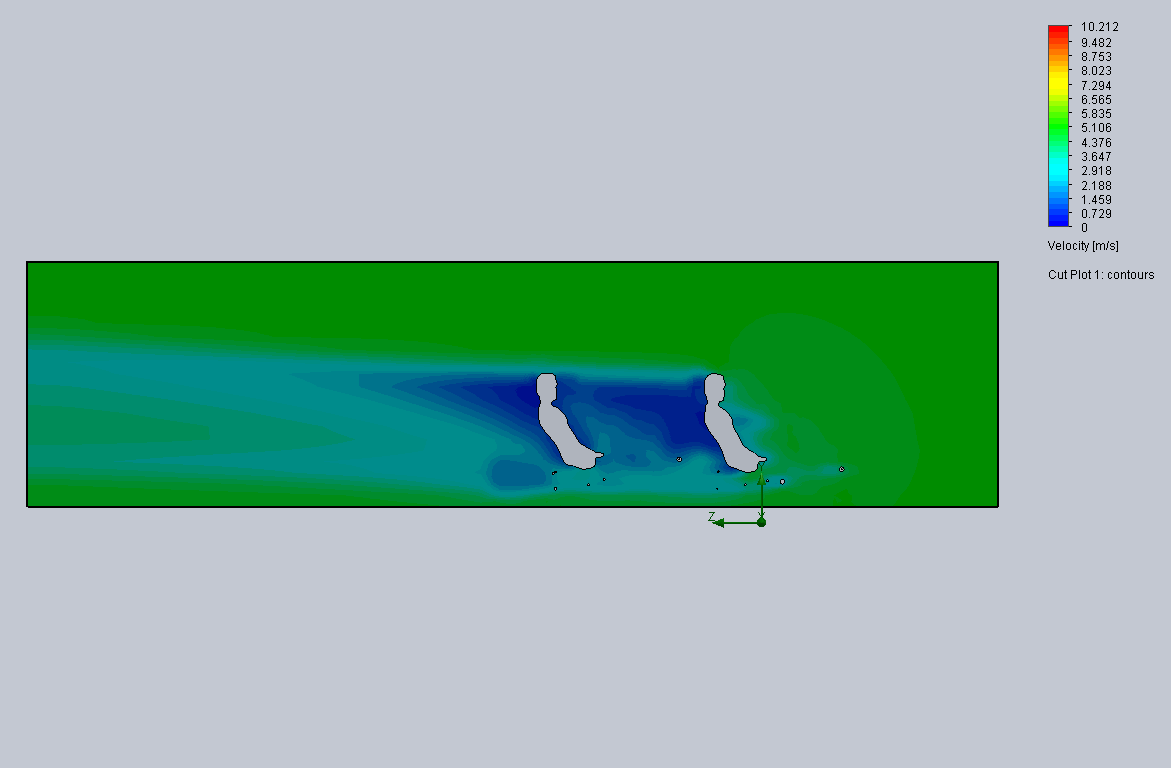
\includegraphics[width=\textwidth]{gm_4_rf_7_v05.png}
\caption{$v = 5 m/s$, global initial mesh = 4}
\end{figure}

\begin{figure}
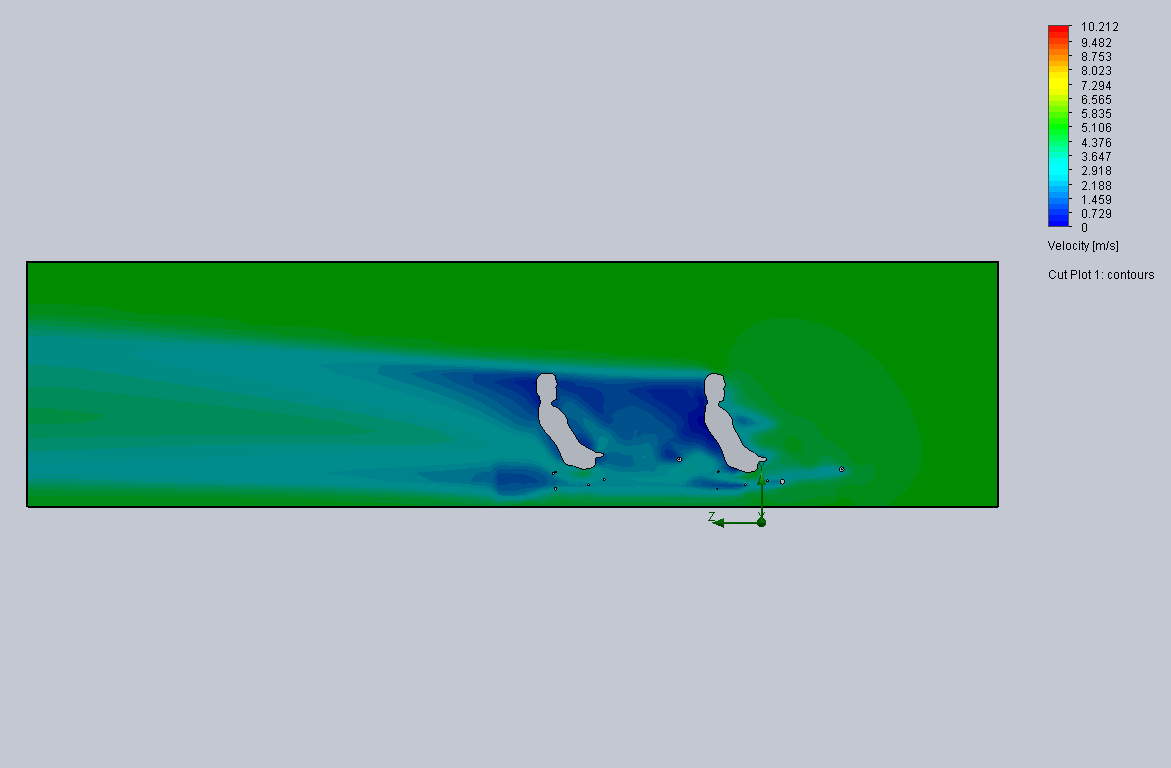
\includegraphics[width=\textwidth]{gm_5_rf_7_v05.png}
\caption{$v = 5 m/s$, global initial mesh = 5}
\end{figure}

\begin{figure}
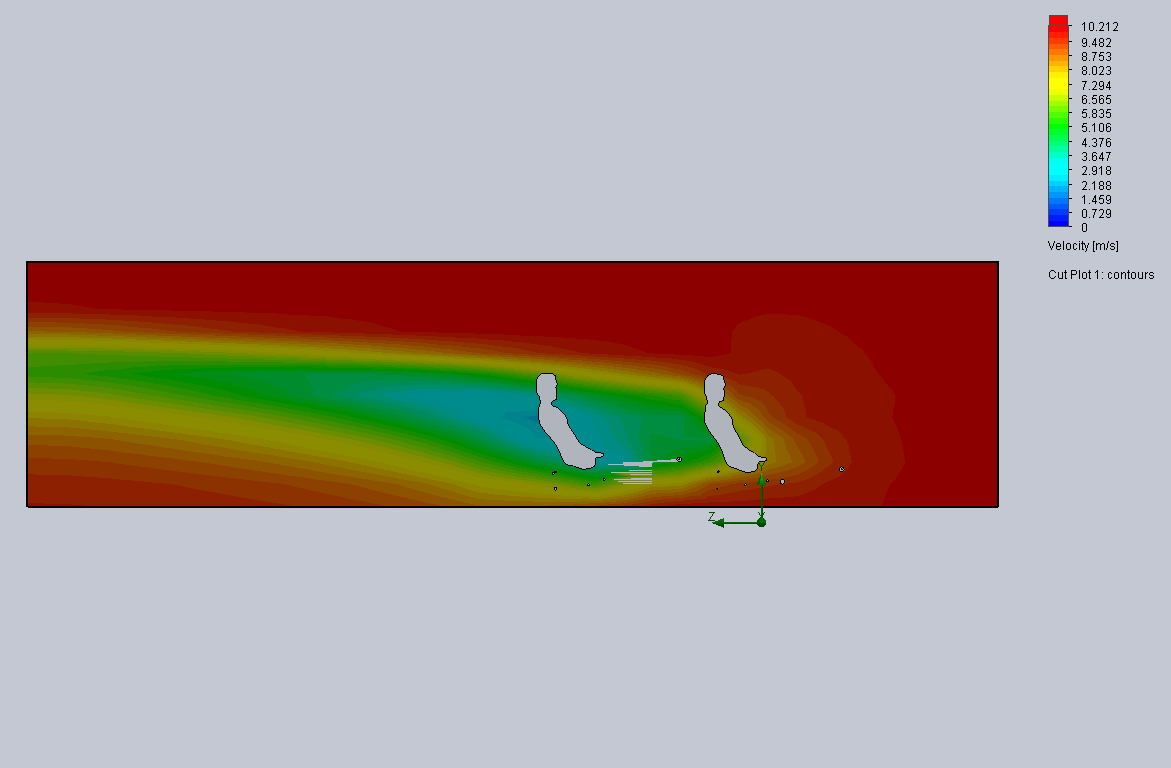
\includegraphics[width=\textwidth]{gm_2_rf_7_v10.png}
\caption{$v = 10 m/s$, global initial mesh = 2}
\end{figure}

\begin{figure}
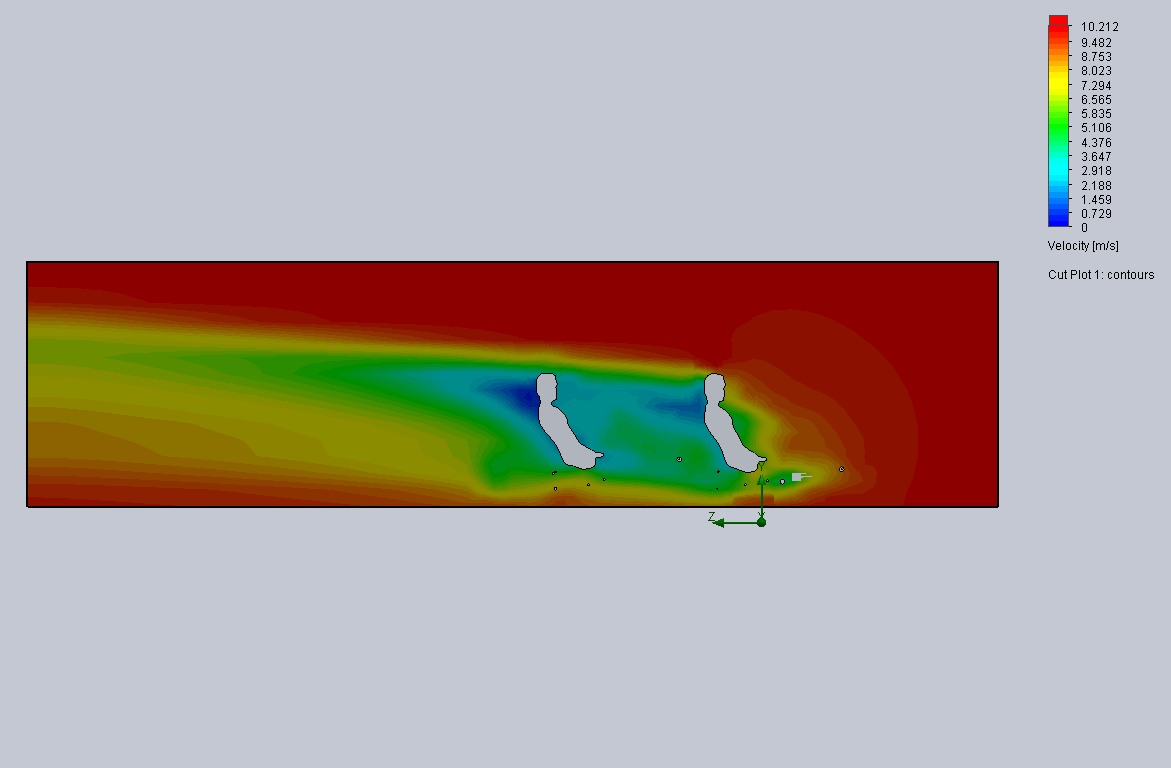
\includegraphics[width=\textwidth]{gm_3_rf_7_v10.png}
\caption{$v = 10 m/s$, global initial mesh = 3}
\end{figure}

\begin{figure}
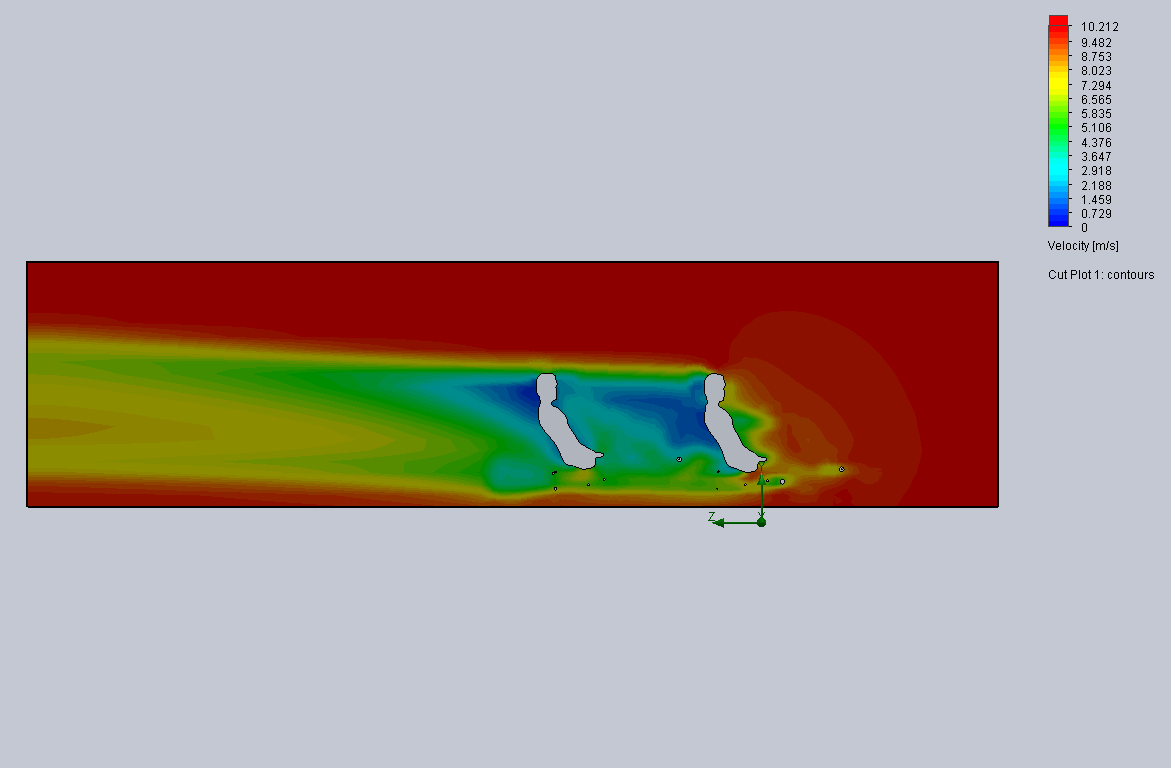
\includegraphics[width=\textwidth]{gm_4_rf_7_v10.png}
\caption{$v = 10 m/s$, global initial mesh = 4}
\end{figure}

\begin{figure}
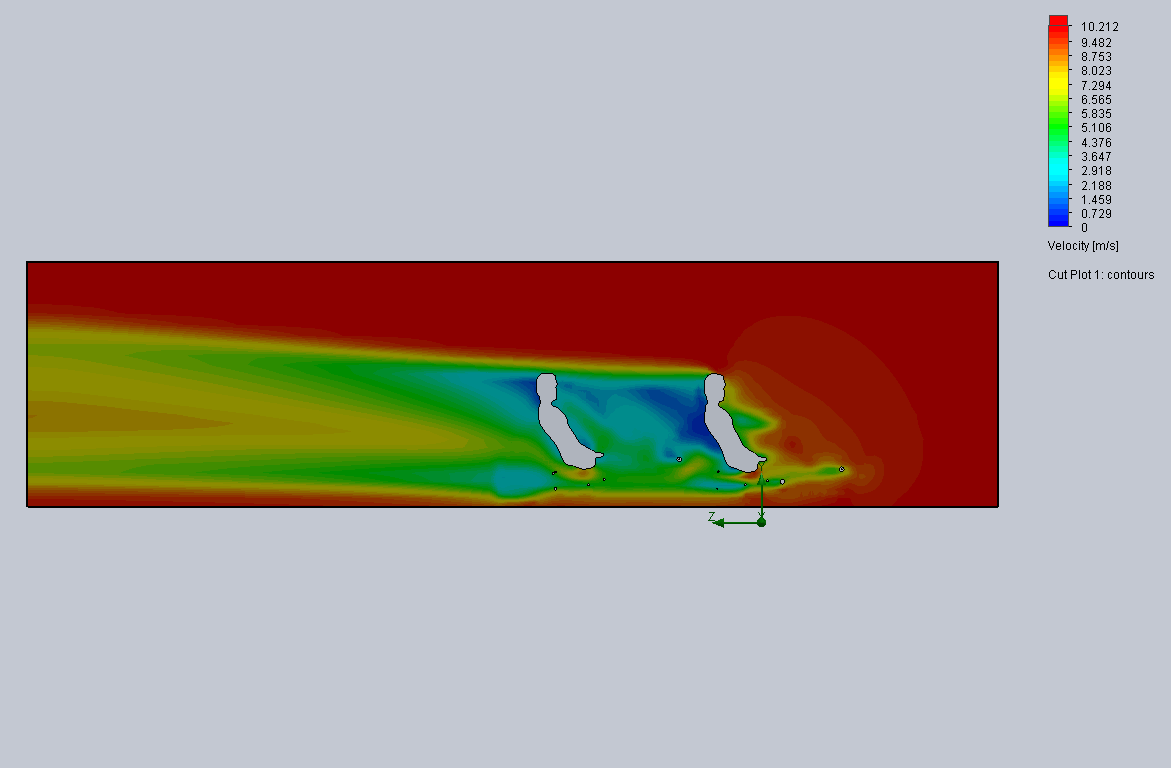
\includegraphics[width=\textwidth]{gm_5_rf_7_v10.png}
\caption{$v = 10 m/s$, global initial mesh = 5}
\end{figure}

\clearpage

\section{roof tests}

\begin{figure}[ht]
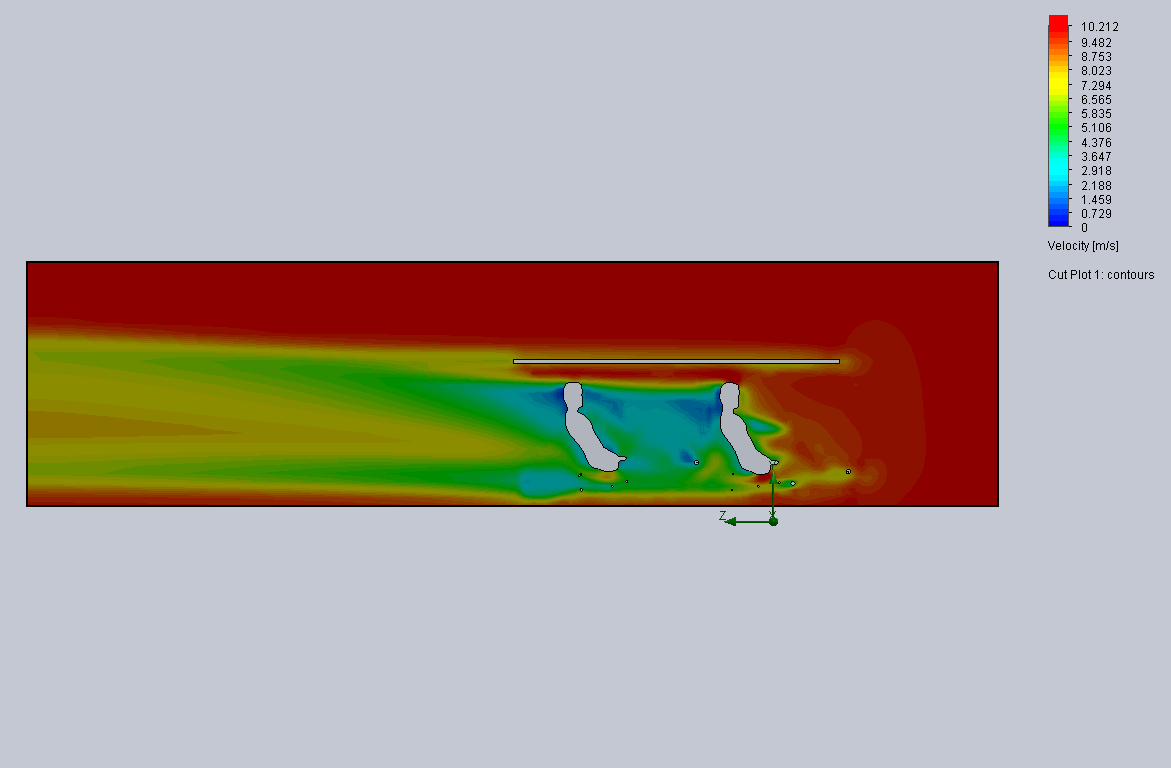
\includegraphics[width=\textwidth]{gm_5_rf_7_v10_roof0.png}
\caption{$v = 10 m/s$, global initial mesh = 5. Note that with the roof the drag increases from 15N to 17N. }
\end{figure}


\begin{figure}[ht]
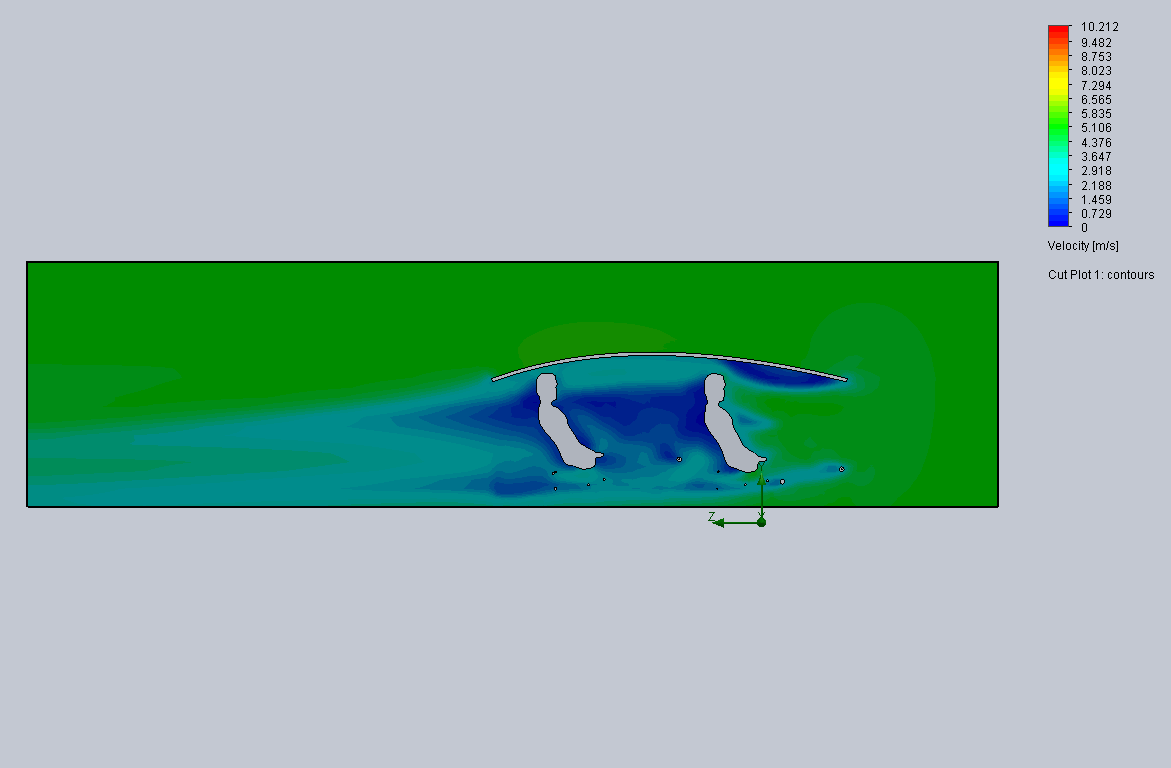
\includegraphics[width=\textwidth]{gm_5_rf_7_v05_roof1.png}
\caption{$v = 5 m/s$, global initial mesh = 5. Note that with the roof the drag increases from 4N to 5N but turbulent tail is significantly suppressed.}
\end{figure}

\begin{figure}[ht]
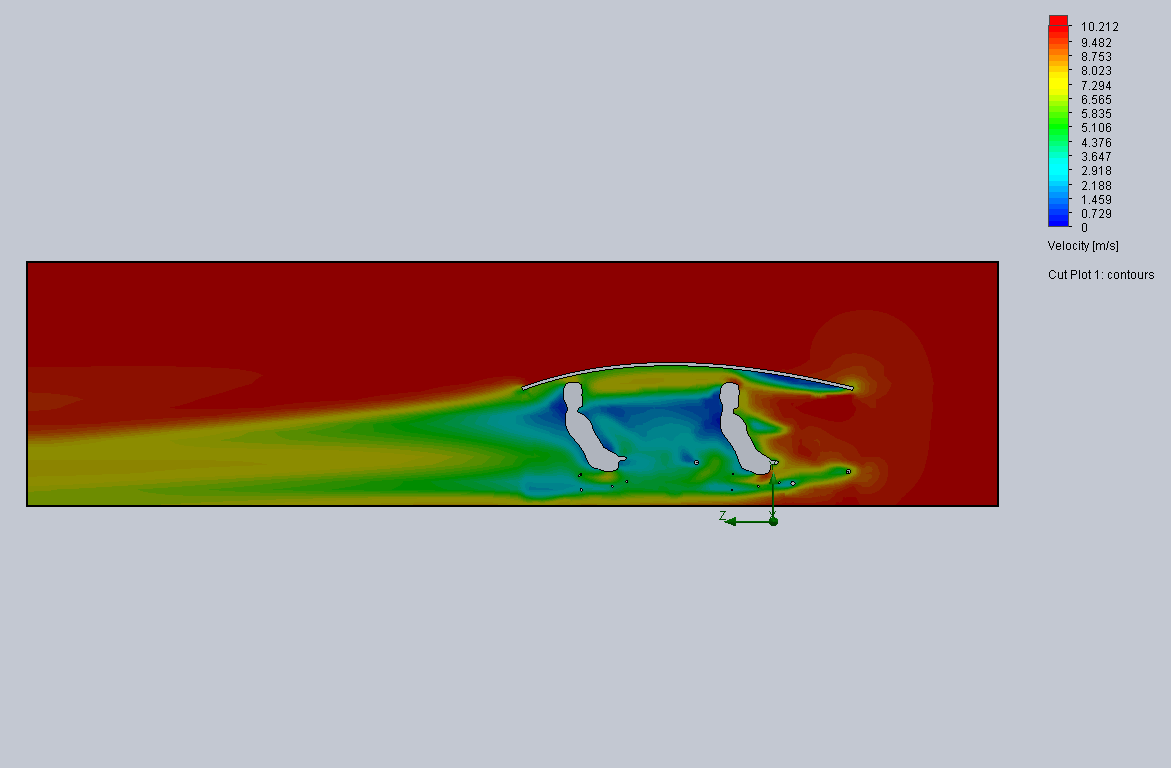
\includegraphics[width=\textwidth]{gm_5_rf_7_v10_roof1.png}
\caption{$v = 10 m/s$, global initial mesh = 5. Note that with the roof the drag increases from 15N to 19N but turbulent tail is significantly suppressed.}
\end{figure}

\begin{figure}[ht]
  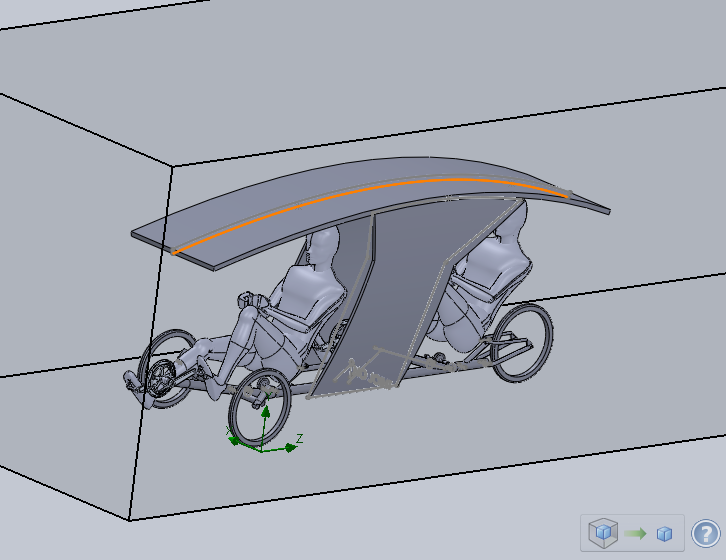
\includegraphics[width=\textwidth]{roof1_sidefender.png}
  \caption{roof and sidefender}
\end{figure}

\begin{figure}[ht]
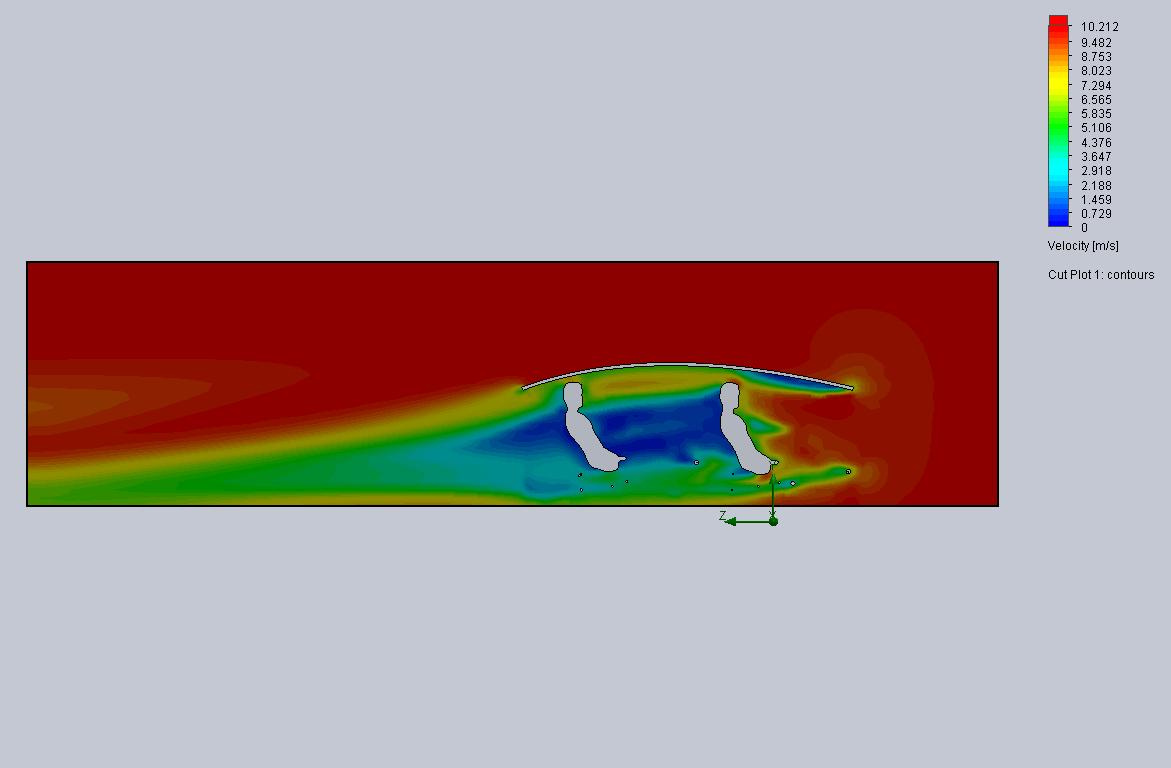
\includegraphics[width=\textwidth]{gm_5_rf_7_v10_roof1_sidefender.png}
\caption{$v = 10 m/s$, global initial mesh = 5. Adding sidefenders reduces drag force from 19N to 18.5N}
\end{figure}


\begin{figure}[ht]
  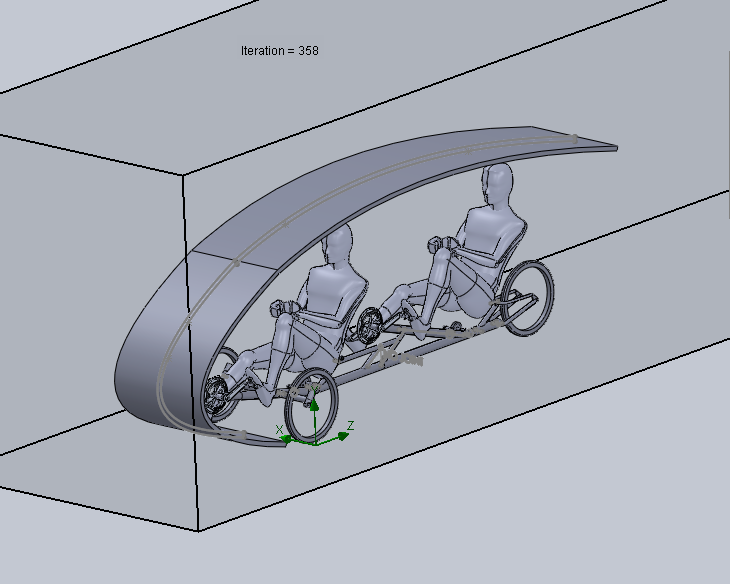
\includegraphics[width=\textwidth]{roof2.png}
  \caption{roof and sidefender}
\end{figure}

\begin{figure}[ht]
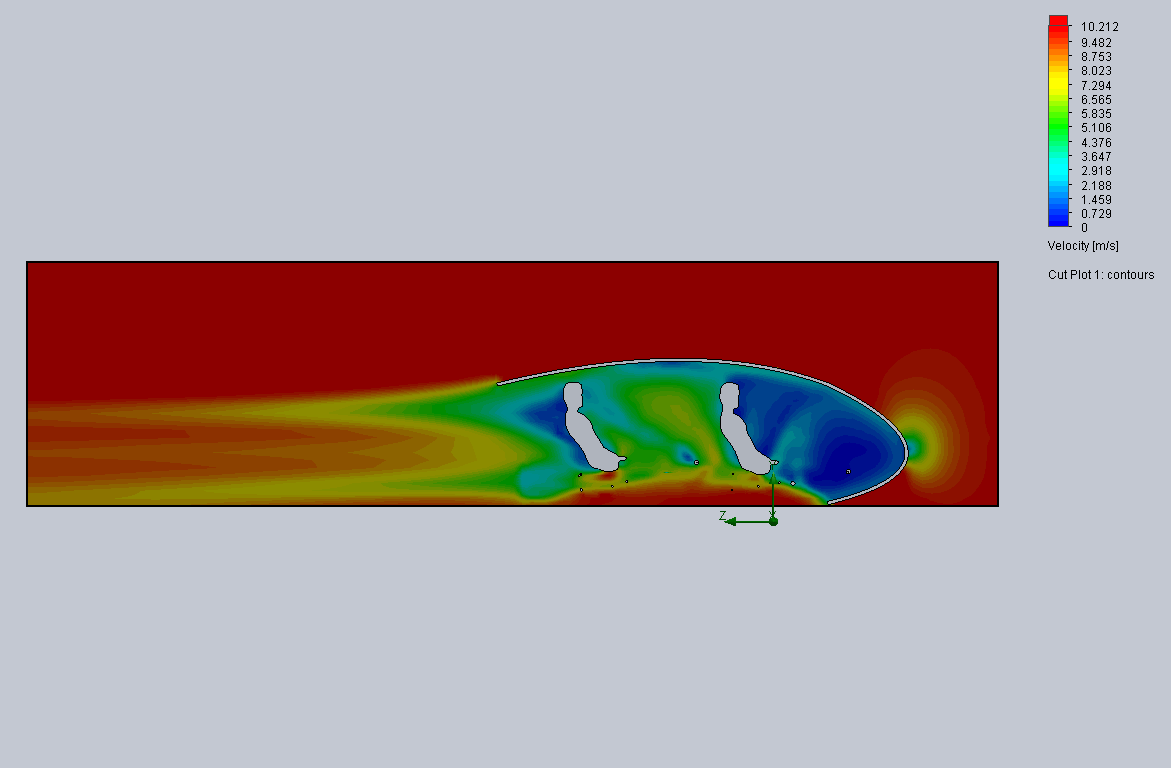
\includegraphics[width=\textwidth]{gm_5_rf_7_v10_roof2.png}
\caption{$v = 10 m/s$, global initial mesh = 5. Drag force is 34N}
\end{figure}

\begin{figure}[ht]
  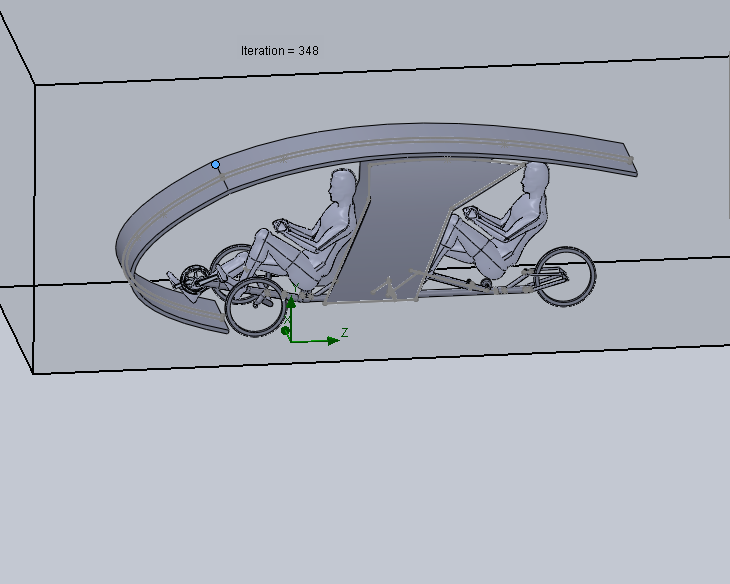
\includegraphics[width=\textwidth]{roof2_sidefender.png}
  \caption{roof and sidefender}
\end{figure}

\begin{figure}[ht]
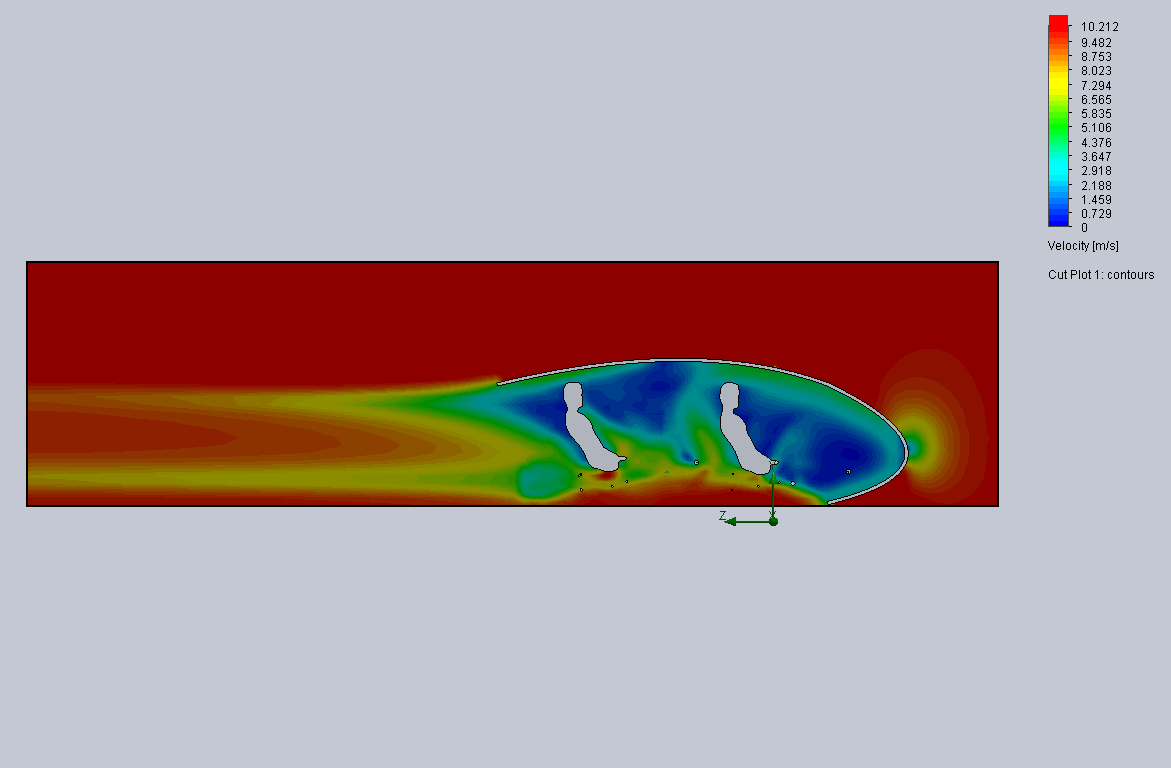
\includegraphics[width=\textwidth]{gm_5_rf_7_v10_roof2_sidefender.png}
\caption{$v = 10 m/s$, global initial mesh = 5. Adding sidefenders reduces drag from 34N to 30N.}
\end{figure}

\end{document}